\chapter{Problema roteamento Veículos com Janelas de Tempo}
\label{cap:Problema_roteamento}

\section{Problema roteamento Veículos com Janelas de Tempo}

Um dos problemas mais famosos de otimização combinatória é o chamado Problema do Caixeiro Viajante, que consiste em determinar o circuito mais curto para se percorrer um dado número de pontos (chamados de nós) e retornar à origem, passando apenas uma vez por cada um deles \cite{lieberman10}. Entretanto, este problema não reflete a realidade da maior parte das organizações, já que estas contam com uma série de veículos, que experimentam diversas restrições (de tempo e capacidade, por exemplo) e percorrem rotas distintas. Logo, o desafio destas empresas é determinar a melhor alocação dos veículos disponíveis, resolvendo um problema de roteamento de veículos (PRV).

O Problema de Roteamento de Veículos (PRV) é descrito como o problema de planejar a entrega ou coleção de rotas ótima. Estas rotas são compostas por veículos que devem partir de um ou vários depósitos para um determinado número de cidades ou clientes espalhados geograficamente, sujeito a um conjunto de restrições.

\cite{laporte92} define o Problema Clássico de Roteamento de Veículos e mostra uma visão geral das diversas abordagens utilizadas para solucioná-lo. Estas se desdobram em algoritmos exatos, que encontram a solução ótima para o problema, e algoritmos heurísticos, que buscam uma boa solução viável, mas que não é necessariamente a solução ótima.

O PRV pode ser definido da seguinte forma: Seja um grafo onde é um conjunto de vértices representando localidades (clientes ou cidades) com o depósito localizado no vértice , e é o conjunto de arcos. Cada arco , é associado a uma matriz de distâncias não negativas. Em alguns contextos, também pode ser interpretado como o custo de viagem ou o tempo de viagem. Quando é simétrico (isto é, a distância/tempo/custo de para é o mesmo de para ), é conveniente substituir por um conjunto de arcos não direcionados. Além disso, assumimos que existem veículos disponíveis no depósito, faz sentido associar um custo fixo ao uso do veículo. Como simplificação, \cite{laporte92} ignorou estes custos, e partiu-se do princípio de que todos os veículos são idênticos e têm a mesma capacidade . O PRV consiste em planejar um conjunto de rotas de menor custo do veículo, de tal forma que:

\begin{itemize}
\item Cada vértice em é visitado apenas uma vez e por exatamente um veículo;
\item Todas as rotas se iniciam e terminam no depósito;
\item As seguintes restrições devem ser respeitadas:
\begin{itemize}
\item Restrição de capacidade: a cada vértice é atribuído um peso não-negativo (ou demanda) e a soma dos pesos de qualquer rota do veículo não pode exceder a capacidade do veículo;
\item O número de vértices em cada rota é limitado a (este é um caso especial de (a) com para todo e );
\item Restrição de tempo total: o comprimento de qualquer rota não pode exceder um limite fixado , sendo este comprimento constituído pelos tempos de viagem e pelos tempos de parada em cada vértice da rota; 
\item Janelas de tempo: o vértice deve ser visitado dentro do intervalo de tempo e é permitido tempo de espera no vértice ;
\item Precedência entre pares de vértices: o vértice pode ter de ser visitado antes do vértice .
\end{itemize}
\end{itemize}


Esta lista não é exaustiva, e uma série de outras variantes interessantes são descritas na literatura.


O Problema de Roteamento de Veículos(PRV) com Janelas de Tempo é uma extensão do PRV onde os serviços de cada cliente devem começar associados a um intervalo de tempo , chamado janela de tempo(\textit{time window}) . As janelas de tempo podem ser rígidas ou flexíveis. em caso de rígida , um veiculo que chega no cliente muito cedo deve esperar até que o cliente esteja pronto para começar o serviço. Em geral , esperar antes do início de uma janela de tempo não incorre em custos. No caso de janelas de tempo flexíveis , cada janela de tempo pode ser violada incorrendo um custo penalização.As janelas de tempo podem ser unilaterais, por exemplo, o tempo máximo para o inicio de uma ação.


Janelas de tempo surgem naturalmente em problemas enfrentados por organizações empresariais que trabalham com horários flexíveis . Problemas específicos com janelas de tempo rígida incluem serviço de segurança e patrulha, entregas bancárias, envios postais, recolhimento de lixo e roteamento de ônibus . Entre os problemas da janela de tempo flexíveis , problemas de entrega de encomendas constituem um exemplo importante. Neste capítulo, vamos nos concentrar principalmente nas Janelas de tempo rígidas.



Na literatura existente sobre o PRVJT , o número de veículos disponíveis para servir os clientes é geralmente considerada ilimitada e a função de objectivo depende da natureza do método de solução escolhida. Para métodos exatos o objetivo é o de minimizar a distância total percorrida. Para heurísticas o principal objetivo é minimizar o número de veículos utilizados e o secundário para minimizar a distância total percorrida. Pode haver excepções a esta declaração geral.



Desde que o PRV é NP-hard , por restrição, PRVJT também é NP-hard \cite{laporte13}.Na verdade até mesmo encontrar uma solução viável para o PRVJT para um número fixo de veículos é em si um problema NP-completo \cite{savelsbergh95}.Uma janela de tempo curta é uma janela que influencia a solução; ou seja, a janela é uma restrição ativa , já as janelas de tempo longas são restrições que influenciam menos nos resultados.



No VRP a geografia é geralmente o fator importante que determina a forma das rotas. Se o número de clientes é pequena, um despachante treinado pode fazer muito bem no planejamento das rotas somente olhando um mapa mostrando a localização dos clientes.No entanto, se a restrição de capacidade é obrigatória para algumas das rotas, é muito mais difícil de ignorar a situação de planejamento.Para o PRVJT quando algumas das rotas são limitadas pela capacidade e outras pelas janelas de tempo, é ainda mais difícil de planejar as rotas manualmente.A interação entre o espaço e os elementos temporais das rotas pode resultar em rotas ótimas que estão longe de a imagem clássica de rotas formadas.Se o número de clientes é aumentada para um nível realista, dizem que pelo menos 100-200, torna-se muito difícil fazer as rotas manualmente. É aqui que os métodos de solução computacionais mostram as suas vantagens\cite{laporte13}.


Os primeiros trabalhos sobre a PRVJT foram estudo de caso orientado \cite{pullen67} e \cite{knight68}. Os métodos de solução com base em heurísticas foram relativamente simples.Os primeiros algoritmos exatos de Branch-and-Bound surgiram no início da década de 1980 \cite{laporte13} e \cite{kolen87}.Em 1987, \cite{solomon87} introduziu instâncias de benchmark envolvendo 100 clientes que foram aceitas como problemas de benchmark padrão pela maioria dos pesquisadores que trabalham no PRVJT e serviu como um catalisador para aumentar a pesquisa sobre o PRVJT.Na década seguinte, muitas heurísticas foram desenvolvidas, as buscas na sua maioria locais, mas também as primeiras metaheurísticas (busca tabu e algoritmos genéticos).Vários algoritmos exatos baseados em metodologias complexas, como relaxamento de Lagrange e de geração de colunas, também foram concebidos.



\section{Formulação Matemática}



O PRVJT é definido no gráfico dirigido G = (V,A) em que o depósito é representado pelos dois vértices 0 e n + 1 , Referido como os vértices partida e destino, respectivamente .Seja N=$V/$\{$0,n+1$\} são o conjunto de vértices do cliente.Todas as rotas de veículos viáveis correspondem caminhos elementares em G.O inverso é, no entanto, não é necessariamente verdade;ou seja, alguns caminhos elementares em G pode não representar rotas viáveis porque violam as janelas de tempo ou a capacidade do veículo.Para simplificar a notação, zero demandas e zero tempos de serviço são definidos para vértices 0 e n + 1 .Além disso, uma janela de tempo está associada com eles exemplo $(a0, b0) = (an+1, bn+1)$ onde a0 e b0 são o mais cedo possível saída do depósito e o último horário possível chegada no depósito,respectivamente .Supondo-se que a matriz de tempo de viagem satisfaz a desigualdade triângulo, existem soluções viáveis apenas se $a_0 \leq min_{i \in V/\{0\})} \{b_i t_{0i}\} $ e $ b_0 \geq max_{i \in V/\{0\})} \{max\{a_0 t_{0i},a_i\}+s_i + t_{i,n+1} \}$




Note que um arco (i,j) $\in$ A pode ser omitida devido a considerações temporais, se $ a_i + s_i + t_{ij} > b_j$ ou limitações de capacidade $ q_i +q_j $ ou por outros fatores.Finalmente, vamos falar que quando os veículos são autorizados a permanecer no depósito, especialmente no caso em que o principal objetivo consiste em minimizar o número de veículos usados, o arco (0,n +1) com $c_{0,n+1 = t_{0,n+1 = 0}} $ deve ser adicionado ao conjunto de arcos A.



Primeiro apresentaremos uma formulação usando Programação Inteira Mista(PIM) para o PRVJT envolvendo dois tipos de variáveis: para cada arco(i,j)$\in$ A e cada veiculo k $\in$ K há um arco variável de fluxo binário $x_{ijk}$ que é igual a 1 se o arco (i, j) é utilizada pelo veículo k, e 0 de outro modo;e, para cada vértice i $\in$ V e veiculo k $\in$ K, temos uma variável de tempo $T_{ik}$ especificando o início do tempo de serviço no vértice i quando servida por veículo k.


O PRVJT pode ser formulado como o seguinte modelo de fluxo de rede de multi-produto com limitações de janela de tempo e de capacidade:

\begin{figure}[ht!]
\centering
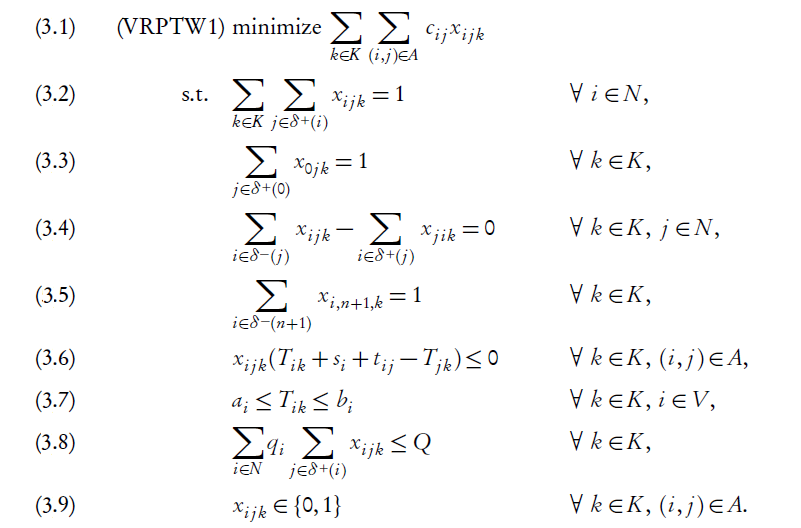
\includegraphics[scale=0.7]{figuras/math1.PNG}
\label{math1}
\end{figure}



função objetivo (3.1) visa minimizar o custo total. As restrições (3.2) garantem que cada cliente é atribuído a exatamente um percurso.Em seguida, as restrições (3.3) - (3.5) definem um caminho da \textit{source-to-sink} no G para cada k veículo.Além disso, as restrições (3.6) - (3.7) e a viabilidade do cronograma (3.8) garantia em relação à janelas de tempo e capacidade do veículo, respetivamente. Finalmente, os arcos de fluxo estão sujeitos a requisitos binários (3.9).

Modelo (3.1) - (3.9) é não linear devido as restrições de (3.6) que pode, no entanto, ser linearizada como: 

\begin{figure}[ht!]
\centering

\includegraphics[scale=0.7]{figuras/math6.PNG}
\label{math6}
\end{figure}

Onde $ M_{ij}$ , (i, j ) $\in$ A, são grandes constantes que podem ser definidas para  $ max \{b_i + s_i +t_{ij} - a_j , 0 \}$



O relaxamento linear do modelo (3.1) - (3.5), (3.6a), (3.7) - (3.9) prevê, em geral, limites inferiores muito fracos . Este modelo tem, no entanto, uma estrutura de bloco-angular que pode ser explorada, onde cada bloco é composto das restrições (3.3) - (3.5), (3.6a), (3.7) - (3.9) para um veículo específico, k $\in$ K e define um Problema do Caminho Mais Curto Elementar com restrições de recursos (ESPPRC). Aplicando o princípio de decomposição de Dantzig-Wolfe \cite{gendreau01} para este modelo produz o seguinte modelo de particionamento definida uma vez que os veículos (idênticos) e suas variáveis correspondentes são agregados \cite{gendreau10}. Neste modelo,$\omega$ denota o conjunto de todas as rotas possíveis, $c_r$ o custo da rota r $\in$ $\omega$ and $a_{ir}$ o número de visitas ao cliente i $\in$ N em rota r $\in$ $\omega$ ($a_{ir}$ $\in$ {0,1}, quando r é uma rota fundamental. Com cada rota r $\in$ $\omega$ está associado um ano variável de caminho binária que assume valor 1 se rota r é selecionado na solução e 0 caso contrário. o modelo de partição do conjunto é

\begin{figure}[ht!]
\centering
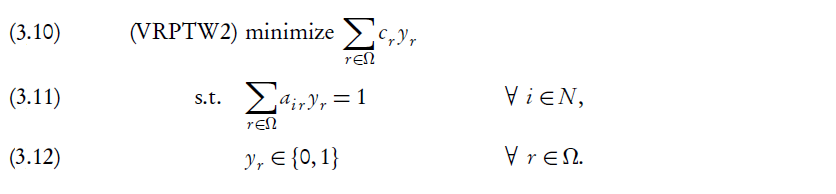
\includegraphics[scale=0.7]{figuras/math2.PNG}
\label{math2}
\end{figure}



função objetivo (3.10) procura minimizar o custo total. Definir restrições de particionamento (3.11) impõem que cada cliente ser visitada apenas uma vez por um veículo. Os requisitos binários nas variáveis caminho de fluxo são expressos por (3.12). Note-se que, como na literatura PRVJT, o modelo acima assume que o número de veículos disponível para atender os clientes é ilimitada, isto é, |k| é tão grande quanto necessário. Se este não foi o caso, a restrição de aplicar a seleção de, no máximo, uma rota disponível por veículo iria ser adicionado ao modelo.

\begin{figure}[ht!]
\centering
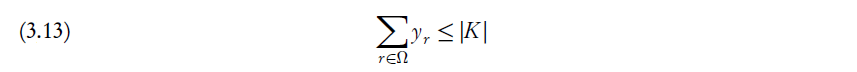
\includegraphics[scale=0.7]{figuras/math3.PNG}
\label{math3}
\end{figure}
 
 
O relaxamento linear do modelo (3.10) - (3.12) produz uma melhor limites mais baixos do que a do modelo (3.1) - (3.5), (3.6a), (3.7) - (3.9). Por outro lado, o modelo de partição do conjunto contém um grande número de variáveis, por rota viável.% No ponto 3.3.1, 

Vários outros modelos foram propostos para a PRVJT. Em particular, as formulações de dois índices foram usados em conjunto com algoritmos Branch-and-CUT . Apresenta-se uma tal formulação abaixo, que envolve um tipo de variáveis: para cada arco (i, j) $\in$ A, existe um binário variável $x_{ij}$ que é igual a 1 se o arco (i, j) é utilizada em solução e 0 se não for usado. Denote por P o conjunto de caminhos (não necessariamente a partir da origem) em G que não respeitam as restrições de janela de tempo e por A (p) o conjunto de arcos no caminho p$\in$ P. Deixe r(S) o número mínimo de veículos necessários para servir cada subconjunto de clientes S de acordo com suas demandas. Este número é, em geral, substituídos por $[q(S)/Q]$ em $q(S)=\sum\limits_{i \in S}q_i $. A formulação de duas índice corresponde à 

\begin{figure}[ht]
\centering
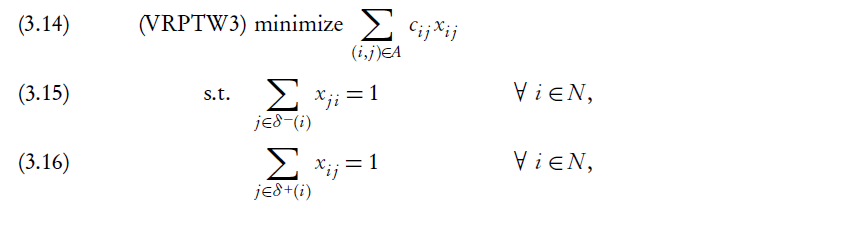
\includegraphics[scale=0.7]{figuras/math4.PNG}
\label{math4}
\end{figure}

\begin{figure}[ht]
\centering
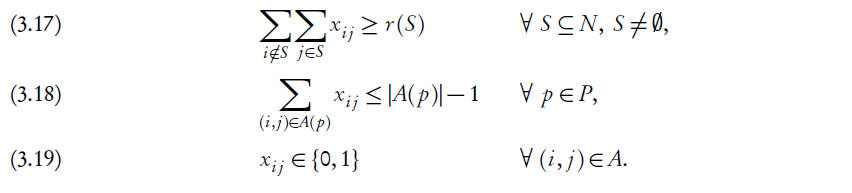
\includegraphics[scale=0.7]{figuras/math5.PNG}
\label{math5}
\end{figure}

função objetivo (3.14) minimiza o custo total para servir os clientes. Restrições (3.15) - (3.16) garantir que um veículo chega e sai de cada cliente, respectivamente. desigualdades de capacidade (3.17) garantir que a capacidade do veículo está satisfeito em todas as rotas selecionadas e também força o relaxamento linear através da imposição de um número mínimo de veículos para atender cada subconjunto de clientes S. Além disso, eles agem como restrições de eliminação sub deslocamento. desigualdades caminho inviável (3.18) proibir a seleção de caminhos que não respeitam as janelas de tempo. Finalmente, as variáveis de fluxo $x_{ij}$ estão sujeitos a requisitos de binários (3.19).

 A formulação de dois índice (3.14) - (3.19) contém um número exponencial de restrições (3.17) e (3.18). Para os casos de tamanhos práticos , eles precisam ser gerados dinamicamente como no algoritmo de plano de corte. desigualdades válidas adicionais também podem ser considerados para apertar o relaxamento linear deste modelo
 


\subsection{Conjunto de Problemas Testes de Solomon}

 O conjunto de problemas teste proposto por Solomon em 1987 \cite{solomon87}, baseado  em  dados  de  alguns  problemas  usados  por  Christofides  et  al.  (1979)  para  o  problema de roteamento padrão, trata-se de diferentes classes de instâncias, cada qual com características   geográficas   e   de   restrições   características.   Os   consumidores   estão   distribuídos em um plano XY de dimensões 100x100.  



As instâncias são divididas em 6 grupos denominados R1, R2, C1, C2, RC1 e RC2. Cada classe contém entre 8 e 12 instâncias. Os grupos R1 e R2, possuem uma disposição geográfica dos clientes de forma aleatória, já nos grupos C1 e C2, a disposição é na forma de  agrupamentos,  e  nos  grupos  RC1  e  RC2  são  tipos  mistos  (parte  em  agrupamentos  e  parte  aleatória).  Nas  classes  R1,  C1  e  RC1,  as  janelas  de  tempo  e  o  horizonte  total  são  curtos, diminuindo assim o número de consumidores por rota. Já as classes R2, C2 e RC2, possuem  um  longo  horizonte  total  fazendo  com  que  as  rotas  tenham  mais  consumidores  viáveis.   


Cada instância tem 100 consumidores, mas pode-se considerar apenas os primeiros 25 ou 50 consumidores dependendo do caso. 



No caso do uso das instâncias de Solomon, nos problemas de roteamento dinâmico, adaptações devem ocorrer para que não se tenha  conhecimento  de  todos  os  consumidores  no início do roteamento, o que tornaria o problema estático.  




%As  figuras  abaixo,  representam  os  três  tipos  de  classe  C  (Fig.2.4),  R  (Fig.2.5)  e    RC(Fig.2.6): 

\begin{figure}[ht!]
	\centering
	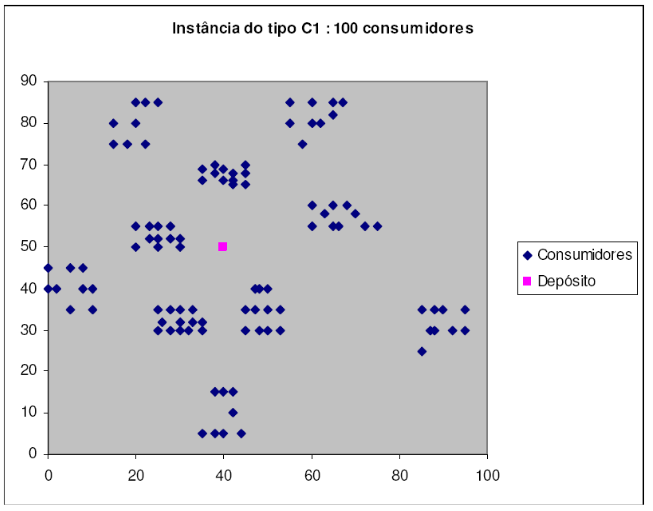
\includegraphics[scale=0.7]{figuras/solo1.PNG}
	\label{solo1}
	\caption{Problemas classe C}
\end{figure}

\begin{figure}[ht!]
	\centering
	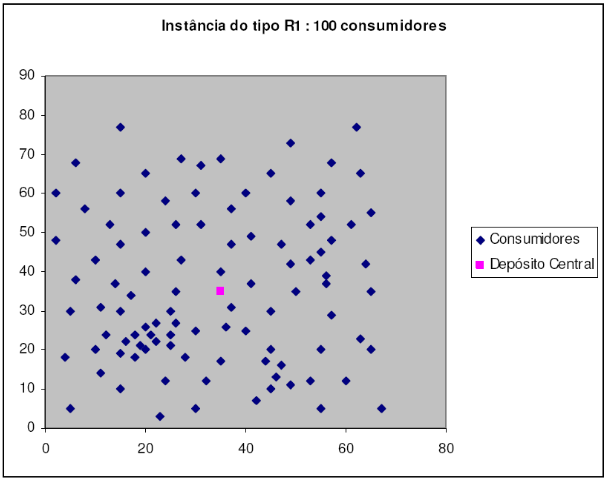
\includegraphics[scale=0.7]{figuras/solo2.PNG}
	\label{solo2}
	\caption{Problemas classe R}
\end{figure}

\begin{figure}[ht!]
	\centering
	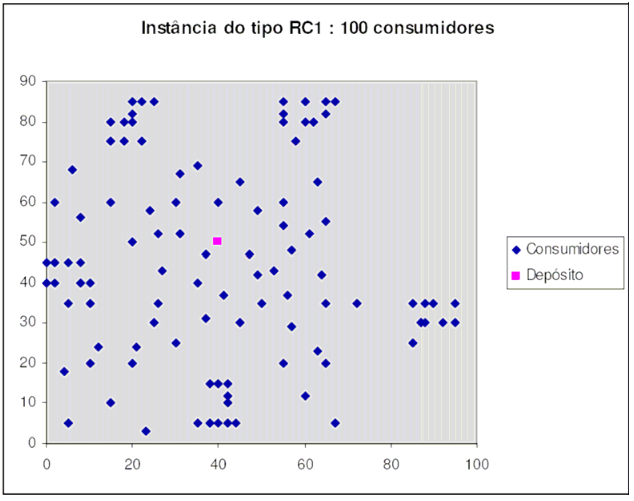
\includegraphics[scale=0.7]{figuras/solo3.PNG}
	\label{solo3}
	\caption{Problemas classe RC}
\end{figure}